%========================{ PACKAGES }=========================

\documentclass[11pt]{article}
% Article type and font.
\usepackage[margin=1in,bottom=1in,top=1in]{geometry}
% Formatting of pages in doc.
\usepackage{setspace}
% Custom control for line spacing in doc.
\usepackage{fancyhdr}
% Fancy Header Pkg.
\usepackage{amsmath}
% American Mathematical Society Math Pkg.
\usepackage{amssymb}
% American Mathematical Society Symbols Pkg.
\usepackage{fdsymbol}
% Many addtnl. mathematical operators.
\usepackage{marvosym}
% Many addtnl. useful symbols, such as for footnotes
\usepackage[dvipsnames]{xcolor}
\definecolor{Lred}{RGB}{255, 102, 102}
\definecolor{bloodorange}{RGB}{255, 83, 0}
\definecolor{Lbloodorange}{RGB}{255, 152, 102}
\definecolor{Lorange}{RGB}{255, 201, 102}
\definecolor{shininggold}{RGB}{255, 210, 0}
\definecolor{Lshininggold}{RGB}{255, 228, 102}
\definecolor{Lyellow}{RGB}{255, 255, 179}
\definecolor{leafgreen}{RGB}{128, 192, 0}
\definecolor{Lleafgreen}{RGB}{179, 217, 102}
\definecolor{hulkgreen}{RGB}{0, 128, 0}
\definecolor{Lhulkgreen}{RGB}{102, 179, 102}
\definecolor{oceanblue}{RGB}{0, 64, 128}
\definecolor{Loceanblue}{RGB}{102, 140, 179}
\definecolor{Lblue}{RGB}{102, 102, 255}
\definecolor{darkblue}{RGB}{38, 0, 193}
\definecolor{Ldarkblue}{RGB}{125, 102, 218}
\definecolor{indigo}{RGB}{75, 0, 130}
\definecolor{Lindigo}{RGB}{147, 102, 180}
\definecolor{codeblack}{RGB}{40, 36, 44}
\definecolor{codeborder}{RGB}{119,136,153}
\definecolor{macosred}{RGB}{255, 92, 84}
\definecolor{macosyellow}{RGB}{252,188,44}
\definecolor{macosgreen}{RGB}{36, 204, 67}
\definecolor{macosgrey}{RGB}{72, 68, 68}
\definecolor{macosblack}{RGB}{28, 28, 28}
\definecolor{apple}{RGB}{67, 199, 51}
\definecolor{electricviolet}{RGB}{106, 65, 246}
\definecolor{blueone}{RGB}{64, 102, 255}
\definecolor{bluetwo}{RGB}{112, 140, 255}
\definecolor{bluethree}{RGB}{160, 179, 255}
\definecolor{bluefour}{RGB}{207, 217, 255}
% more colors & some custom ones (L = light)
\usepackage{tikz}
% Manually draw math pictures using code
\usepackage{multicol}
% Split page into multiple columns
\usetikzlibrary{positioning}
% Useful for manually-creating graphs (e.g. lattices).
\usepackage{graphicx}
\graphicspath{ {./images/} }
% Upload images directly into doc, size them, etc.
% Uploaded images are pulled from ./images/ folder in sidebar.
\usepackage[font=small,labelfont=bf]{caption}
% Create custom captions for images, graphs, etc.
\usepackage{multirow}
\setlength{\columnseprule}{1pt}
\setlength{\columnsep}{20pt}
\def\columnseprulecolor{\color{black}}
% For tables
\usepackage{colortbl}
% For coloring cells of tables
\usepackage{arydshln}
% For dashed lines surrounding cells in tables
\usepackage[]{mdframed}
% Creates box around text: useful for code/solutions.
\usepackage{hyperref}
\hypersetup{hidelinks}
% Hyperlinks; second one makes their clickable boxes invisible
\usepackage{booktabs}
% For style lines dividing matrix elements inside.
\usepackage{textcomp}
% For straight, single quotes.
\usepackage{yfonts}
% adds fonts like gothic
% 11-color rainbow palette
\usepackage{longfbox}
\makeatletter
\newdimen\@tempdimd
\makeatother
\usepackage[many]{tcolorbox}
% for rounded boxes around text
% highlighting text (colorful)
\tcbuselibrary{skins, xparse, listings}
% for something to do with the realisitc command shell
\usepackage{pgfornament}
% for decorative symbols and such
\usepackage{array}
% need this for something table-related


%====================={ CUSTOM COMMANDS }===================== 

\newcommand{\Mod}[1]{\ (\mathrm{mod}\ #1)}
% Modular Arithmetic spacing + parenthesis
\NewDocumentCommand{\Customarrow}{}{\hspace{0.2cm}\rightarrow\hspace{0.2cm}}
% Large custom "implies" arrow
\NewDocumentCommand{\customarrow}{}{\hspace{0.1cm}\rightarrow\hspace{0.1cm}}
% Small custom "implies" arrow
\NewDocumentCommand{\newproblem}{mm}
{\begin{center}
    \section*{\underline{Problem #1:{}{#2}}}
\end{center}}
% New Problem: formatting, bolding, spacing, etc.
\NewDocumentCommand{\problempart}{mm}{\noindent\textbf{(#1){ } #2}}
% Part x of Problem y

\def\barroman#1{\sbox0{#1}\dimen0=\dimexpr\wd0+1pt\relax
  \makebox[\dimen0]{\rlap{\vrule width\dimen0 height 0.09ex depth 0.06ex}%
    \rlap{\vrule width\dimen0 height\dimexpr\ht0+0.06ex\relax 
            depth\dimexpr-\ht0+0.09ex\relax}%
    \kern.5pt#1\kern.5pt}}
% Roman Numerals: \barroman{letter(s)}

\newtcolorbox{redbox}[1]{colback=red!5!white,
colframe=red,fonttitle=\bfseries,
title={#1}}
% red text box

\newtcolorbox{bloodorangebox}[1]{colback=bloodorange!5!white,
colframe=bloodorange,fonttitle=\bfseries,
title={#1}}
% bloodorange text box

\newtcolorbox{orangebox}[1]{colback=orange!5!white,
colframe=orange,fonttitle=\bfseries,
title={#1}}
% orange text box

\newtcolorbox{shininggoldbox}[1]{colback=shininggold!5!white,
colframe=shininggold,fonttitle=\bfseries,
title={#1}}
% shininggold text box

\newtcolorbox{yellowbox}[1]{colback=yellow!5!white,
colframe=yellow,fonttitle=\bfseries,
title={#1}}
% yellow text box

\newtcolorbox{leafgreenbox}[1]{colback=leafgreen!5!white,
colframe=leafgreen,fonttitle=\bfseries,
title={#1}}
% leafgreen text box

\newtcolorbox{hulkgreenbox}[1]{colback=hulkgreen!5!white,
colframe=hulkgreen,fonttitle=\bfseries,
title={#1}}
% hulkgreen text box

\newtcolorbox{oceanbluebox}[1]{colback=oceanblue!5!white,
colframe=oceanblue,fonttitle=\bfseries,
title={#1}}
% oceanblue text box

\newtcolorbox{bluebox}[1]{colback=blue!5!white,
colframe=blue,fonttitle=\bfseries,
title={#1}}
% blue text box

\newtcolorbox{darkbluebox}[1]{colback=darkblue!5!white,
colframe=darkblue,fonttitle=\bfseries,
title={#1}}
% darkblue text box

\newtcolorbox{indigobox}[1]{colback=indigo!5!white,
colframe=indigo,fonttitle=\bfseries,
title={#1}}
% indigo text box

\newtcolorbox{blackbox}[1]{colback=black!5!white,
colframe=black,fonttitle=\bfseries,
title={#1}}
% black text box

\newcommand\codebox[1]{
    \noindent\hspace{-0.25em}\begin{tcolorbox}[on line, hbox, colback = codeblack, colframe = codeborder, coltext = white, boxrule = 1.5pt, left = 2pt, right = 2pt, top = 0.5pt, bottom = 0.5pt]
    \small\texttt{#1}\normalsize
    \end{tcolorbox}
}
% for typesetting console commands

    \newtcblisting{MacTerminal}{colback=macosblack, colupper=white, colframe=macosgrey, listing only,
        listing options={style=tcblatex,language=sh,escapeinside=``,},
        title={\vspace{0.25em}\hspace{-1em}\textcolor{macosred}{\Huge{$\bullet$}}\textcolor{macosyellow}{\Huge{$\bullet$}}\textcolor{macosgreen}{\Huge{$\bullet$}}},
        every listing line={\MyMacTerminalPrompt}}
        \pgfkeys{/MacTerminal/.cd,
        user/.code={\gdef\MyMacTerminalUser{#1}},user={},
        host/.code={\gdef\MyMacTerminalHost{#1}},host={},
        color/.code={\gdef\MyMacTerminalColor{#1}},color=white,
        prompt char/.code={\gdef\MyMacTerminalPromptChar{#1}},prompt char=\%,
        root/.style={user=anthonymalysz,host=@Air,color=white,prompt char=\%},
        bob/.style={user=bob,host=@remotehost,color=cyan},
        }
        
    \newcommand{\SU}[1]{\pgfkeys{/MacTerminal/.cd,#1}
    \gdef\MyMacTerminalPrompt{\textcolor{\MyMacTerminalColor}{\small\ttfamily\bfseries \MyMacTerminalUser\MyMacTerminalHost{}\hspace{0.2cm}\textcolor{white}{\url{~}}\hspace{0.2cm}{\textcolor{white}\MyMacTerminalPromptChar}}}}
    \newcommand{\StartConsole}{\gdef\MyMacTerminalPrompt{}}

    \SU{user=anthonymalysz,host=@Air,color=white}

    % `\SU{bob}`
    % whoami`\StartConsole`
    % bob`\SU{bob}`
    % _
% for drawing realistic mac terminal window; commented out part is for 2nd user 'Bob'

    \newtcblisting{ubuntu}{colback=macosblack, colupper=white, colframe=macosgrey, listing only,
        listing options={style=tcblatex,language=sh,escapeinside=``,},
        title={\vspace{0.25em}\hspace{-1em}\textcolor{macosred}{\Huge{$\bullet$}}\textcolor{macosyellow}{\Huge{$\bullet$}}\textcolor{macosgreen}{\Huge{$\bullet$}}},
        every listing line={\MyUbuntuPrompt}}
        \pgfkeys{/ubuntu/.cd,
        user/.code={\gdef\MyUbuntuUser{#1}},user={},
        host/.code={\gdef\MyUbuntuHost{#1}},host={},
        color/.code={\gdef\MyUbuntuColor{#1}},color=white,
        prompt char/.code={\gdef\MyUbuntuPromptChar{#1}},prompt char=\$,
        root/.style={user=ubuntu,host=@primary,color=apple,prompt char=\$},
        bob/.style={user=bob,host=@remotehost,color=cyan},
        }
        
    \newcommand{\switchuser}[1]{\pgfkeys{/ubuntu/.cd,#1}
    \gdef\MyUbuntuPrompt{\textcolor{\MyUbuntuColor}{\small\ttfamily\bfseries \MyubuntuUser\MyUbuntuHost{\textcolor{white}{:}}\textcolor{electricviolet}{\large{$\sim$}}{\textcolor{white}\MyUbuntuPromptChar}}}}
    \newcommand{\BeginConsole}{\gdef\MyUbuntuPrompt{}}

    \switchuser{user=ubuntu,host=ubuntu@primary,color=apple}

    % `\SU{bob}`
    % whoami`\StartConsole`
    % bob`\SU{bob}`
    % _
% for drawing realistic Ubuntu terminal window; commented out part is for 2nd user 'Bob'

%========================{ DOCUMENT }=========================

\onehalfspacing
\begin{document}

\begin{blackbox}{\begin{center}\Large\textbf{Table of Contents:}\end{center}}
\begin{center}\large\textit{In Progress...}\end{center}

\large\textbf{\hyperlink{page.1}{Work Log}} ................................................................................................................ \hyperlink{page.1}{1}\\
\large\textbf{\hyperlink{page.2}{Communications \& Ideas Pad}} ............................................................................. \hyperlink{page.2}{2}
\end{blackbox}

\begin{blackbox}{\begin{center}\Large\textbf{Work Log:}\end{center}}
\hspace{-0.3cm}\small\textbf{\hyperlink{page.3}{WEEK [I.]}}
\vspace{0.25em}

\normalsize\indent \vline\textbf{------------}\hyperlink{page.3}{\fcolorbox{red}{white}{Mon 05/22}}\textbf{------}\hyperlink{page.3}{\fcolorbox{red}{white}{Tue 05/23}}\textbf{------}\hyperlink{page.5}{\fcolorbox{red}{white}{Wed 05/24}}\textbf{------}\hyperlink{page.7}{\fcolorbox{red}{white}{Thrs 05/25}}\textbf{------}\hyperlink{page.7}{\fcolorbox{red}{white}{Fri 05/26}} \\

\vspace{-1em}
\hspace{-0.3cm}\small\textbf{\hyperlink{page.8}{WEEK [II.]}}
\vspace{0.25em}

\normalsize\indent \vline\textbf{------------}\fbox{\hspace{0.28cm}Holiday\hspace{0.28cm}}\textbf{------}\hyperlink{page.8}{\fcolorbox{bloodorange}{white}{Tue 05/30}}\textbf{------}\hyperlink{page.10}{\fcolorbox{bloodorange}{white}{Wed 05/31}}\textbf{------}\hyperlink{page.11}{\fcolorbox{bloodorange}{white}{Thrs 06/01}}\textbf{------}\hyperlink{page.13}{\fcolorbox{bloodorange}{white}{Fri 06/02}} \\

\vspace{-1em}
\hspace{-0.3cm}\small\hyperlink{page.14}{\textbf{WEEK [III.]}}
\vspace{0.25em}

\normalsize\indent \vline\textbf{------------}\hyperlink{page.14}{\fcolorbox{orange}{white}{Mon 06/05}}\textbf{------}\hyperlink{page.15}{\fcolorbox{orange}{white}{Tue 06/06}}\textbf{------}\fcolorbox{orange}{white}{Wed 06/07}\textbf{------}\fcolorbox{orange}{white}{Thrs 06/08}\textbf{------}\fcolorbox{orange}{white}{Fri 06/09} \\

\vspace{-1em}
\hspace{-0.3cm}\small\textbf{WEEK [VI.]}
\vspace{0.25em}

\normalsize\indent \vline\textbf{------------}\fcolorbox{shininggold}{white}{Mon 06/12}\textbf{------}\fcolorbox{shininggold}{white}{Tue 06/13}\textbf{------}\fcolorbox{shininggold}{white}{Wed 06/14}\textbf{------}\fcolorbox{shininggold}{white}{Thrs 06/15}\textbf{------}\fcolorbox{shininggold}{white}{Fri 06/16} \\

\vspace{-1em}
\hspace{-0.3cm}\small\textbf{WEEK [V.]}
\vspace{0.25em}

\normalsize\indent \vline\textbf{------------}\fcolorbox{yellow}{white}{Mon 06/19}\textbf{------}\fcolorbox{yellow}{white}{Tue 06/20}\textbf{------}\fbox{\hspace{0.28cm}Holiday\hspace{0.28cm}}\textbf{------}\fcolorbox{yellow}{white}{Thrs 06/22}\textbf{------}\fcolorbox{yellow}{white}{Fri 06/23} \\

\vspace{-1em}
\hspace{-0.3cm}\small\textbf{WEEK [VI.]}
\vspace{0.25em}

\normalsize\indent \vline\textbf{------------}\fcolorbox{leafgreen}{white}{Mon 06/26}\textbf{------}\fcolorbox{leafgreen}{white}{Tue 06/27}\textbf{------}\fcolorbox{leafgreen}{white}{Wed 06/28}\textbf{------}\fcolorbox{leafgreen}{white}{Thrs 06/29}\textbf{------}\fcolorbox{leafgreen}{white}{Fri 06/30} \\

\vspace{-1em}
\hspace{-0.3cm}\small\textbf{WEEK [VII.]}
\vspace{0.25em}

\normalsize\indent \vline\textbf{------------}\fcolorbox{hulkgreen}{white}{Mon 07/03}\textbf{------}\fbox{\hspace{0.22cm}Holiday\hspace{0.22cm}}\textbf{------}\fcolorbox{hulkgreen}{white}{Wed 07/05}\textbf{------}\fcolorbox{hulkgreen}{white}{Thrs 07/06}\textbf{------}\fcolorbox{hulkgreen}{white}{Fri 07/07} \\

\vspace{-1em}
\hspace{-0.3cm}\small\textbf{WEEK [VIII.]}
\vspace{0.25em}

\normalsize\indent \vline\textbf{------------}\fcolorbox{oceanblue}{white}{Mon 07/10}\textbf{------}\fcolorbox{oceanblue}{white}{Tue 07/11}\textbf{------}\fcolorbox{oceanblue}{white}{Wed 07/12}\textbf{------}\fcolorbox{oceanblue}{white}{Thrs 07/13}\textbf{------}\fcolorbox{oceanblue}{white}{Fri 07/14} \\

\vspace{-1em}
\hspace{-0.3cm}\small\textbf{WEEK [IX.]}
\vspace{0.25em}

\normalsize\indent \vline\textbf{------------}\fcolorbox{blue}{white}{Mon 07/17}\textbf{------}\fcolorbox{blue}{white}{Tue 07/18}\textbf{------}\fcolorbox{blue}{white}{Wed 07/19}\textbf{------}\fcolorbox{blue}{white}{Thrs 07/20}\textbf{------}\fcolorbox{blue}{white}{Fri 07/21} \\

\vspace{-1em}
\hspace{-0.3cm}\small\textbf{WEEK [X.]}
\vspace{0.25em}

\normalsize\indent \vline\textbf{------------}\fcolorbox{darkblue}{white}{Mon 07/24}\textbf{------}\fcolorbox{darkblue}{white}{Tue 07/25}\textbf{------}\fcolorbox{darkblue}{white}{Wed 07/26}\textbf{------}\fcolorbox{darkblue}{white}{Thrs 07/27}\textbf{------}\fcolorbox{darkblue}{white}{Fri 07/28} \\

\vspace{-1em}
\hspace{-0.3cm}\small\textbf{WEEK [XI.]}
\vspace{0.25em}

\normalsize\indent \vline\textbf{------------}\fcolorbox{indigo}{white}{Mon 07/31}\textbf{------}\fcolorbox{indigo}{white}{Tue 08/01}\textbf{------}\fcolorbox{indigo}{white}{Wed 08/02}\textbf{------}\fbox{\textbf{PRESENTATION}}
\end{blackbox}
\newpage

%========================={ HEADER }==========================

\pagestyle{fancy}
\fancyhead[L]{\textbf{NIST SURF Program}}
\fancyhead[C]{\hspace{-1.5cm} Malysz, Stein}
\fancyhead[R]{\textbf{May 22nd - August 3rd, 2023}}

%=========================={ BODY }===========================

\begin{tcbraster}[%
    raster columns=1,
    raster rows=1,
    code={%
      \tcbheightfromgroup\topboxheight{topbox}%
      \tcbheightfromgroup\bottomboxheight{bottombox}%
    },
    raster height=\textheight-\topboxheight-\bottomboxheight-4mm]{\begin{center}\Large\textbf{Communications \& Ideas Pad:}\end{center}}
    \begin{tcolorbox}
        \begin{itemize}
            \item TYPE HERE what comes across the noggin...
            \item ...
            \item ...
        \end{itemize}
    \end{tcolorbox}
\end{tcbraster}

\newpage

\noindent\begin{longfbox}[
rounded,
padding=4pt,
border-width=1.5pt,
border-top-left-radius=30pt,
border-left-width=8pt,
border-color=red,
background-color=Lred,
border-right-style=double,
]
\medskip
\phantom{~~}\Large\textbf{WEEK \barroman{I}.} \large(05/22 - 05/26)\phantom{~~~~~~~~~~~~~~~~~~~~~~~~~~~~~~~~~~~~~}\large\textbf{\textit{Getting Comfortable...}}
\end{longfbox}
\\

\begin{center}
\vspace{-1em}
\pgfornament[color=red, width=6cm, ydelta=-10pt]{88}
\vspace{-0.5em}
\end{center}

\normalsize\begin{redbox}{Monday, May 22nd\vspace{-2em}\begin{flushright}\large\textbf{Orientation}\end{flushright}}
\begin{itemize}
    \item Attended welcome meeting via BlueJeans.
    \item Sat in on a meeting of AJ's with people reporting their week's work in the NIST ITL.
\end{itemize}
\end{redbox}

\begin{center}
\pgfornament[color=red,width=1cm,ydelta=-10pt]{11}\pgfornament[color=red,width=0.5cm,ydelta=-10pt]{6}\pgfornament[color=red,width=1cm,ydelta=-10pt]{14}
\vspace{-0.5em}
\end{center}

\begin{redbox}{Tuesday, May 23rd\vspace{-2em}\begin{flushright}\large\textbf{VM Struggles}\end{flushright}}
\begin{itemize}
    \item Had trouble with iTAC getting into my work laptop; installed VirtualBox with the goal of installing Ubuntu as the VM inside it. Decided using homebrew would be easier.
    \item Installed multipass using \codebox{brew install multipass}.
    \item Confirmed it worked by running \codebox{multipass version} and \codebox{multipass find}:
    \begin{MacTerminal}
 multipass version`\StartConsole`
multipass   1.10.1+mac 
multipassd  1.10.1+mac 
    
########################################################################
Multipass 1.11.1 bug fix release
Fix Windows path, Virtualbox mount failure, Windows native mounts

Go here for more information: 
https://github.com/canonical/multipass/releases/tag/v1.11.1
########################################################################`\SU{root}`
\end{MacTerminal}
\end{itemize}
\begin{center}
\textbf{\large\bullet} \\
\textbf{\large\bullet} \\
\textbf{\large\bullet} \\
\large\textbf{\textit{Continued}...} \\
\textbf{\large\bullet} \\
\textbf{\large\bullet} \\
\textbf{\large\bullet} \\
\end{center}
\end{redbox}

\begin{redbox}{Tuesday, May 23rd (cont. \#1/2)}
\begin{MacTerminal}
 multipass find `\StartConsole` 
Image                   Aliases      Version     Description
18.04                   bionic       20230525    Ubuntu 18.04 LTS
20.04                   focal        20230523    Ubuntu 20.04 LTS
22.04                   jammy,lts    20230518    Ubuntu 22.04 LTS
anbox-cloud-appliance                latest      Anbox Cloud Appliance
charm-dev                            latest      A development and 
                                                 testing environment 
                                                 for charmers
docker                               0.4         A Docker environment 
                                                 with Portainer and 
                                                 related tools
jellyfin                             latest      Jellyfin is a Free 
                                                 Software Media System 
                                                 that puts you in 
                                                 control of managing 
                                                 and streaming your 
                                                 media.
minikube                             latest      minikube is local 
                                                 Kubernetes
ros-noetic                           0.1         A development and 
                                                 testing environment 
                                                 for ROS Noetic.
ros2-humble                          0.1         A development and 
                                                 testing environment 
                                                 for ROS 2 Humble.`\SU{root}`
    
    \end{MacTerminal}
\begin{itemize}
    \item Proceeded to follow \href{https://medium.com/@paulrobu/how-to-run-ubuntu-22-04-vms-on-apple-m1-arm-based-systems-for-free-c8283fb38309}{\textbf{this blog}} to figure out how to run Ubuntu 22.04 VMs on my Apple M1 ARM-based system for free, whose steps included:
    \begin{enumerate}
        \item\codebox{multipass launch 22.04 -n primary -c 2 -m 4G -d 16G}
        \item\codebox{multipass shell}
        \item\codebox{sudo passwd ubuntu}
    \end{enumerate}
    To access the newly-installed desktop, I discovered the IP address of the VM by running \codebox{ip a}within the Ubuntu shell. I then used the IP address, and to connect I downloaded Microsoft Remote Desktop from the AppStore. Not sure if it worked.
    \begin{center}
        \large\textbf{(\textit{Continued} ...)}
    \end{center}
\end{itemize}
\end{redbox}
\begin{redbox}{Tuesday, May 23rd (cont. \#2/2)}
\begin{itemize}
    \item Spent a bit more time figuring out how to run a web server on a multipass VM (on macOS with an M1 processor), mostly using StackOverflow and prompting ChatGPT (I think I was successful, as I was able to visit the IP address at the end in my browser):
    \begin{enumerate}
    \item\large\textbf{Installation: }\normalsize Install Multipass by visiting the Multipass website (https://multipass.run/) and downloading the appropriate version for macOS M1. Follow the provided instructions to complete the installation.
    \item\large\textbf{Launching a Multipass VM: }\normalsize Launch a Multipass VM by opening a terminal window and running \codebox{multipass launch --name my-vm}. This will create a new virtual machine named \texttt{my-vm}. 
    \item\large\textbf{Accessing the VM: }\normalsize To access the Multipass VM, run \codebox{multipass shell my-vm}. This will open a shell session inside the VM. 
    \item\large\textbf{Installing and Configuring the Web Server: }\normalsize Install Apache inside the VM by running \codebox{sudo apt update} and \codebox{sudo apt install apache2}. Once the installation is complete, Apache should be running automatically. You can test it by opening a web browser on your Mac and navigating to \texttt{http://<VM-IP-address>}. Replace \texttt{<VM-IP-address>} with the IP address of your Multipass VM.
    \item\large\textbf{Sharing Files with the VM: }\normalsize By default, the Multipass VM doesn't have direct access to your Mac's file system. You can use the Multipass file transfer feature to share files between your Mac and the VM. To transfer files from your Mac to the VM, use the following command: \codebox{multipass transfer /path/to/local/file my-vm:/path/to/destination/file}, (for me, the \texttt{/path/to/destination/file} was \texttt{/Users/anthonymalysz}). To transfer files from the VM to your Mac, use the following command: \codebox{multipass transfer my-vm:/path/to/vm/file /path/to/destination/file}. Replace the paths with the appropriate locations on your Mac and the VM. 
    \end{enumerate}
\end{itemize}
\end{redbox}

\begin{center}
\pgfornament[color=red,width=1cm,ydelta=-10pt]{11}\pgfornament[color=red,width=0.5cm,ydelta=-10pt]{6}\pgfornament[color=red,width=1cm,ydelta=-10pt]{14}
\vspace{-0.5em}
\end{center}

\begin{redbox}{Wednesday, May 24th\vspace{-2em}\begin{flushright}\large\textbf{Firewall Struggles}\end{flushright}}
\begin{itemize}
    \item Started the day by figuring out how to configure two HTTP servers, one on port 8080 and one on port 9090 by opening two shells and running \codebox{python3 -m http.server 8080} in one shell and \codebox{python3 -m http.server 9090} in the other; then, I installed \href{https://en.wikipedia.org/wiki/Iptables}{\textbf{iptables}} and configured the iptables such that access to the 9090 HTTP server was allowed, but access to the 8080 server was prohibited. These were the steps I took (ChatGPT, SO):
\end{itemize}
\end{redbox}

\begin{redbox}{Wednesday, May 24th (cont. \#1/2)}
\begin{itemize}
    \begin{itemize}
        \item Open up two terminal windows and run \codebox{python3 -m http.server 8080} and \codebox{python3 -m http.server 9090}, so that they're both up.
        \item Create a new Apache configuration file for the first server on port 8080: \codebox{sudo nano /etc/apache2/other/first\_server.conf}. This command will create a new configuration file specifically for the first server.
        \item Inside this file, I added the following configuration (then I saved the changes by pressing Ctrl + X, then Y, then Enter) and exited the editor:
        \end{itemize}
        \begin{MacTerminal}
 sudo nano /etc/apache2/other/first_server.conf `\StartConsole`

Listen 8080
<VirtualHost *:8080>
    DocumentRoot "/Users/anthonymalysz"
</VirtualHost>`\SU{root}`
        \end{MacTerminal}
    \begin{itemize}
        \item Similarly, I created a new Apache configuration file for the second server on port 9090 by running: \codebox{sudo nano /etc/apache2/other/second\_server.conf}. This command created a new configuration file specifically for the second server.
        \item Inside the file, I added the following configuration (then I saved the changes by pressing Ctrl + X, then Y, then Enter) and exited the editor:
        \end{itemize}
        \begin{MacTerminal}
 sudo nano /etc/apache2/other/second_server.conf `\StartConsole`

Listen 9090
<VirtualHost *:9090>
    DocumentRoot "/Users/anthonymalysz"
</VirtualHost>`\SU{root}`
        \end{MacTerminal}
    \begin{itemize}
        \item At this point, I've created separate configuration files for each server on ports 8080 and 9090, which are stored in \codebox{/etc/apache2/other/first\_server.conf} and \codebox{/etc/apache2/other/second\_server.conf}, respectively. 
        \item Next, I installed \codebox{pf} (Packet Filter) as a firewall. I edited the \codebox{pf} configuration file and added the following two lines to the bottom:
    \end{itemize}
\end{itemize}
\end{redbox}
\begin{redbox}{Wednesday, May 24th (cont. \#2/2)}
    \begin{MacTerminal}
 sudo nano /etc/pf.conf`\StartConsole`

rdr pass inet proto tcp from any to any port 9090 -> 127.0.0.1 port 9090
block in inet proto tcp from any to any port 8080
    \end{MacTerminal}
\begin{itemize}
    \begin{itemize}
        \item After saving changes and exiting, I enabled \codebox{pf} by running \codebox{sudo pfctl -e}.
    \end{itemize}
    \item After seeing that I could still access both by visiting \codebox{http://localhost:8080} and \codebox{http://localhost:9090}, it seems that I was supposed to do all of this inside the Ubuntu VM to begin with...oops! In any case, this was more of a learning experience than anything to begin with, to see how these things are still done more ``manually" than they ``should" be. 
    \item During our sync meeting for the day, we decided to avoid things like this in the future---and to have better strucutre and records overall going forward---that we should create a \LaTeX document to log all of our work.
\end{itemize}
\end{redbox}

\begin{center}
\pgfornament[color=red,width=1cm,ydelta=-10pt]{11}\pgfornament[color=red,width=0.5cm,ydelta=-10pt]{6}\pgfornament[color=red,width=1cm,ydelta=-10pt]{14}
\vspace{-0.5em}
\end{center}

\begin{redbox}{Thursday, May 25th\vspace{-2em}\begin{flushright}\large\textbf{Documentation Begins}\end{flushright}}
\begin{itemize}
    \item Spent the whole day creating this document from scratch, getting it to a point where all weeks' text boxes are colored, styled, and ready to be written in; also, see new sections \hyperlink{page.1}{\textbf{Work Log}} and \hyperlink{page.1}{\textbf{Table of Contents}} (works in progress) with clickable hyperlinks to other pages (you can only see these by hovering over them, but I'll try to make it obvious when links are link-y). Will share with AJ soon, so that this can become a collaborative document to mostly log progress, but also to communicate ideas/concerns/goals.
\end{itemize}
\end{redbox}

\begin{center}
\pgfornament[color=red,width=1cm,ydelta=-10pt]{11}\pgfornament[color=red,width=0.5cm,ydelta=-10pt]{6}\pgfornament[color=red,width=1cm,ydelta=-10pt]{14}
\vspace{-0.5em}
\end{center}

\begin{redbox}{Friday, May 26th\vspace{-2em}\begin{flushright}\large\textbf{Catch-Up}\end{flushright}}
\begin{itemize}
    \item Gained access to my NIST Laptop and downloaded necessary apps.
    \item Filled in Monday's, Tuesday's, and Wednesday's activities in this document (using Element DMs, ChatGPT prompt history, and Internset search history), and made new commands that will help with typesetting code and realisic-looking terminal window(s). 
    \item Explored our \href{https://github.com/users/aj-stein-nist/projects/2}{\textbf{GitHub Project Board}}, linked Overleaf with public GitHub repo.
\end{itemize}
\end{redbox}
\newpage

\noindent\begin{longfbox}[
rounded,
padding=4pt,
border-width=1.5pt,
border-top-left-radius=30pt,
border-left-width=8pt,
border-color=bloodorange,
background-color=Lbloodorange,
border-right-style=double,
]
\medskip
\phantom{~~}\Large\textbf{WEEK \barroman{II}.} \large(05/30 - 06/02)\phantom{~~~~~~~~~~~~~~~~~~~~~~~~~~~~~~~~~~~~~~~~~~~~}\large\textbf{\textit{Network Protocols}}
\end{longfbox}
\\

\begin{center}
\vspace{-1em}
\pgfornament[color=bloodorange, width=6cm, ydelta=-10pt]{88}
\vspace{-0.5em}
\end{center}

\normalsize\begin{bloodorangebox}{Tuesday, May 30th\vspace{-2em}\begin{flushright}\large\textbf{Success with \texttt{iptables}}\end{flushright}}
\begin{itemize}
    \item We refreshed what we did last week, and tried to see if I could run a Linux VM on my work laptop, now that it's accessible. Trying to run Powershell on Windows 10 as administrator (administrative command prompt) didn't work, as I needed a user/login from NIST. Trying to run the command \codebox{usl --install} in a normal Powershell prompt didn't work either, with the same result. We'll try to resolve this issue by filing a waiver (asking for permission, in the government bureaucracy) to NIST.
    \item In the meantime, on my Mac I tried repeating all of last week's shenanigans with \codebox{iptables}, only this time actually in the Linux VM:
    \begin{itemize}
        \item Similar to before, we open two terminal windows and run \codebox{multipass shell} to access the Ubuntu shell. We then host HTTP servers on ports 8080 and 9000, using \codebox{python3 -m http.server 8080}and \codebox{python3 -m http.server 9000}.
        \item Like in last week's demo, upon opening a third terminal window and accessing the Ubuntu shell, running \codebox{sudo iptables -L -n} brings up the current list of network policies on this Linux VM, which are all set to \texttt{ACCEPT} by default:
\begin{ubuntu}
 sudo iptables -L -n`\BeginConsole`
Chain INPUT (policy ACCEPT)
target     prot opt source               destination         

Chain FORWARD (policy ACCEPT)
target     prot opt source               destination         

Chain OUTPUT (policy ACCEPT)
target     prot opt source               destination    
\end{ubuntu}
        \item After running \codebox{sudo iptables -A INPUT -p tcp --dport 8080 -j ACCEPT} and \codebox{sudo iptables -A INPUT -p tcp --dport 9000 -j DROP}, we can check this list of policies again and see that two new ``rows'' have been added:
    \end{itemize}
\end{itemize}

\begin{center}
\vspace{0.5em}
\large\textbf{(\textit{Continued}...)} \\
\vspace{1.5em}
\end{center}
\end{bloodorangebox}

\newpage
\begin{bloodorangebox}{Tuesday, May 30th (Cont. \#1/1)}
\begin{ubuntu}
Chain INPUT (policy ACCEPT)
target     prot opt source               destination         
ACCEPT     tcp  --  0.0.0.0/0            0.0.0.0/0            tcp dpt:8080
DROP       tcp  --  0.0.0.0/0            0.0.0.0/0            tcp dpt:9000

Chain FORWARD (policy ACCEPT)
target     prot opt source               destination         

Chain OUTPUT (policy ACCEPT)
target     prot opt source               destination    
\end{ubuntu}

\begin{itemize}
    \begin{itemize}
        \item By typing \codebox{ip a} and checking what the IP address is (in this case, it's not \codebox{localhost} like I tried last time---we will hopefully go over what \texttt{localhost} is later), we visit \codebox{http://192.168.64.3:8080} and \codebox{http://192.168.64.3:9000} (where the IP address is \codebox{192.168.64.3}). If done correctly, we should now be able to visit the former page, but not the latter.
        \item\textbf{Note:} to delete (flush) any changes we've made to the network policies on our VM, we can run \codebox{sudo iptables -F} to flush the firewall rules.
    \end{itemize}
    \item Investigated what different \href{https://en.wikipedia.org/wiki/Category:Transport_layer_protocols}{\textbf{transport layer protocols}} are, and how I think a computer is able to distinguish them (so that I can make a firewall treat each differently):
    \end{itemize}
    \begin{multicols}{2}
        Every \textbf{packet} follows a 5-layer structure:
        \begin{itemize}
            \item\textbf{Application} $\longrightarrow$ HTTP
            \vspace{-0.2cm}\item\textbf{Transport} $\longrightarrow$ TCP, UDP, ...
            \vspace{-0.2cm}\item\textbf{Network} $\longrightarrow$ IP
            \vspace{-0.2cm}\item\textbf{Link} $\longrightarrow$ WiFi
            \vspace{-0.2cm}\item\textbf{Physical} $\longrightarrow$ Ethernet Cable
        \end{itemize}
        The \textbf{Transport Layer} allows simultaneous use of a network connection by multiple applications. When the \textbf{Application Layer} creates a message, it is sent to the Transport Layer, which then wraps it in a \textbf{segment}: it includes additional information like source port and destination port. The segment is then sent to the \textbf{Network Layer}.
        \vfill
        \columnbreak
        \scriptsize\textbf{TCP:} transmits packets in a streamlined, numbered fashion; even if they arrive out-of-order, they will be re-arranged before reception by another application. TCP uses a congestion protocol to handle high-traffic networks, so while slower and with more overhead space, it makes sense where there's greater bandwidth; an effect of this, though, is less control over when packets are sent. With TCP, re-transmission is possible and also secured by a 3-way handshake: Network A asks Network B to set up a connection, Network B responds, and finally Network A communicates the established connection. TCP might be used to stream videos or send pictures and texts. \\
        \hline
        \vspace{0.75em}
        \scriptsize\textbf{UDP:} transmits packets in a discrete fashion, without order and prioritizing efficiency over reliability or security: useful in instances of low bandwidth, or if packets are mutually uncorrelated. When using UDP, packet loss is much more common as well; packets are only sent once, so if they are lost in transmission, they simply go discarded, unannounced. UDP might be used to send emails or play online video games (packet loss $>$ lag).
    \end{multicols}
\end{bloodorangebox}

\begin{center}
\pgfornament[color=bloodorange,width=1cm,ydelta=-10pt]{11}\pgfornament[color=bloodorange,width=0.5cm,ydelta=-10pt]{6}\pgfornament[color=bloodorange,width=1cm,ydelta=-10pt]{14}
\vspace{-0.5em}
\end{center}

\begin{bloodorangebox}{Wednesday, May 31st\vspace{-2em}\begin{flushright}\large\textbf{Investigating Protocols}\end{flushright}}
\begin{center}
\vspace{-0.5em}
\resizebox{14cm}{2.46cm}{\hspace{0.5cm}
\begin{tabular}{lccl}
\multicolumn{1}{c}{}                                  & \textbf{\begin{tabular}[c]{@{}c@{}}\small{TCP/IP Model (1982)}\end{tabular}} & \textbf{\begin{tabular}[c]{@{}c@{}}\small{OSI Model (1984)}\end{tabular}} &  \\ \cline{2-3}
\multicolumn{1}{l|}{\multirow{3}{*}{\raisebox{-4ex}[0ex][0ex]{\scriptsize{HTTP, SSH, FTP, ...}}}} & \multicolumn{1}{c|}{\multirow{3}{*}{\textbf{APPLICATION}}}             & \multicolumn{1}{c|}{\cellcolor{blueone}APPLICATION}                                    &  \\ \cdashline{3-3}
\multicolumn{1}{l|}{}                                 & \multicolumn{1}{c|}{}                                                  & \multicolumn{1}{c|}{\cellcolor{blueone}PRESENTATION}                                   &  \\ \cdashline{3-3}
\multicolumn{1}{l|}{}                                 & \multicolumn{1}{c|}{}                                                  & \multicolumn{1}{c|}{\cellcolor{blueone}SESSION}                                        &  \\ \cdashline{1-1}\cline{2-3}
\multicolumn{1}{l|}{\raisebox{-0.5ex}[0ex][0ex]{\scriptsize{TCP, UDP, ...}}}                         & \multicolumn{1}{c|}{\textbf{TRANSPORT}}                                & \multicolumn{1}{c|}
{\cellcolor{bluetwo}TRANSPORT}                                      &  \\ \cdashline{1-1}\cline{2-3}
\multicolumn{1}{l|}{\raisebox{-0.5ex}[0ex][0ex]{\scriptsize{Ethernet, Switches, ...}}}               & \multicolumn{1}{c|}{\textbf{INTERNET}}                                 & \multicolumn{1}{c|}{\cellcolor{bluethree}NETWORK}                                        &  \\ \cdashline{1-1}\cline{2-3}
\multicolumn{1}{l|}{\multirow{2}{*}{\raisebox{-2ex}[0ex][0ex]{\scriptsize{Cables, NIC, ...}}}}     & \multicolumn{1}{c|}{\multirow{2}{*}{\textbf{LINK}}}                    & \multicolumn{1}{c|}{\cellcolor{bluefour}DATA LINK}                                      &  \\ \cdashline{3-3}
\multicolumn{1}{l|}{}                                 & \multicolumn{1}{c|}{}                                                  & \multicolumn{1}{c|}{\cellcolor{bluefour}PHYSICAL}                                       &  \\ \cdashline{1-1}\cline{2-3}
\end{tabular}
}
\end{center}
\vspace{-0.5em}
$$\big\Downarrow\hspace{5cm}\big\Downarrow\hspace{5 cm}\big\Downarrow\hspace{0.7cm}$$
\begin{tabular}{|m{0.10\textwidth}|m{0.13\textwidth}|m{0.685\textwidth}|}
\cline{1-3}
\textbf{\begin{tabular}[c]{@{}c@{}}\hspace{0.1cm}\large{HTTP}\end{tabular}}       & \hspace{0.06cm}\cellcolor{blueone}\footnotesize{\textbf{Application}} & \tiny{\textbf{Hypertext Transfer Protocol} is the foundation of the World Wide Web, and is used to load webpages using hypertext links. HTTP is an application layer protocol designed to transfer information between networked devices and runs on top of other layers of the network protocol stack. In a typical flow over HTTP, a client machine makes a request---these have a version type, URL, method, request headers, and (optional) body---to a server, which then responds.}                                                                                                                                                                                                                                                                                                                                                                                                                                                                                                                                                                                                                                                                                                                                                               \\ \cline{1-1} \cline{3-3} 
\textbf{\begin{tabular}[c]{@{}c@{}}\hspace{0.3cm}\large{SSH}\end{tabular}}                       & \hspace{0.06cm}\cellcolor{blueone}\footnotesize{\textbf{Application}} & \tiny{\textbf{Secure Shell} is a cryptographic network protocol for operating network services securely over unsecured networks. Its most notable applications are remote login and command-line execution. SSH applications are based on a client–server architecture, connecting an SSH client instance with an SSH server. SSH operates as a layered protocol suite with three principal hierarchical components: the transport layer provides server authentication, confidentiality, and integrity; the user authentication protocol validates the user to the server; and the connection protocol multiplexes the encrypted tunnel into multiple logical communication channels.}                                                                                                                                                                                                                                                                                                                                                                                                                                                                                                                                                                                                                                                                                                                                                                \\ \cline{1-1} \cline{3-3} 
\textbf{\begin{tabular}[c]{@{}c@{}}\hspace{0.3cm}\large{FTP}\end{tabular}}             & \hspace{0.06cm}\cellcolor{blueone}\footnotesize{\textbf{Application}} & \tiny{\textbf{File Transfer Protocol} is a standard communication protocol used for the transfer of computer files from a server to a client on a computer network. FTP is built on a client–server model architecture using separate control and data connections between the client and the server. FTP users may authenticate themselves with a clear-text sign-in protocol, usually with a username and password, but can connect anonymously if the server is configured to allow it. FTP is often secured with SSL/TLS or replaced with SSH File Transfer Protocol.}                                                                                                                                                                                                                                                                                                                                                                                                                                              \\ \cline{1-1} \cline{3-3} 
\textbf{\begin{tabular}[c]{@{}c@{}}\hspace{0.26cm}\large{TCP}\end{tabular}}      & \hspace{0.18cm}\cellcolor{bluetwo}\footnotesize{\textbf{Transport}}   & \tiny{\textbf{Transmission Control Protocol} is one of the main protocols of the IP suite. \hyperlink{page.9}{\textbf{[See Above]}}}                                                                                                                                                                                                                                                                                                                                                                                                                                                                                                                                                                                                                                                                                                                                                         \\ \cline{1-1} \cline{3-3} 
\textbf{\begin{tabular}[c]{@{}c@{}}\hspace{0.24cm}\large{UDP}\end{tabular}}             & \hspace{0.18cm}\cellcolor{bluetwo}\footnotesize{\textbf{Transport}}   & \tiny{\textbf{User Datagram Protocol} is one of the core communication protocols of the Internet protocol suite used to send messages to other hosts on an IP network. \hyperlink{page.9}{\textbf{[See Above]}}}                                                                                                                                                                                                                                                                                                                                                                                                                                                                                                                                                                                                                                                                                                                                 \\ \cline{1-1} \cline{3-3} 
\textbf{\begin{tabular}[c]{@{}c@{}}\hspace{0.55cm}\large{IP}\end{tabular}}                   & \hspace{0.32cm}\cellcolor{bluethree}\footnotesize{\textbf{Internet}}    & \tiny{\textbf{Internet Protocol} is the network layer communications protocol for relaying datagrams across network boundaries. Its routing function enables internetworking, and essentially establishes the Internet. IP has the task of delivering packets from the source host to the destination host solely based on the IP addresses in the packet headers. For this purpose, IP defines packet structures that encapsulate the data to be delivered. It also defines addressing methods that are used to label the datagram with source and destination information. The original Internet Protocol Version 4 (IPv4) is the dominant protocol of the Internet, with successor IPv6.}                                                                                                                                                                                                                                                                                                                                                                                                                                                                                                                                                                                                                                                                                                                                                                 \\ \cline{1-1} \cline{3-3} 
\textbf{\begin{tabular}[c]{@{}c@{}}\hspace{0.15cm}\large{ICMP}\end{tabular}} & \hspace{0.32cm}\cellcolor{bluethree}\footnotesize{\textbf{Internet}}    & \tiny{\textbf{Internet Control Message Protocol} is used by network devices (e.g. router), to send error messages and operational info. indicating (un)successful communications with another IP address. ICMP differs from transport protocols (TCP, UDP, etc.) in that it is not typically used to exchange data between systems nor regularly employed by end-user network applications.}                                                                                                                                                                                                                                                                                                                                                                                                                                                                                                                                                                                                                                                                                                                                                               \\ \cline{1-1} \cline{3-3} 
\textbf{\begin{tabular}[c]{@{}c@{}}\hspace{0.25cm}\large{ARP}\end{tabular}}        & \hspace{0.32cm}\cellcolor{bluethree}\footnotesize{\textbf{Internet}}    & \tiny{\textbf{Address Resolution Protocol} is a communication protocol that discovers the link layer address (e.g. MAC address) associated with a given internet layer address (usually IPv4).}                                                                                                                                                                                                                                                                                                                                                                                                                                                                                                                                                                                                                                                                                                                                                                \\ \cline{1-1} \cline{3-3} 
\textbf{\begin{tabular}[c]{@{}c@{}}\small{Ethernet}\end{tabular}}       & \hspace{0.61cm}\cellcolor{bluefour}\footnotesize{\textbf{Link}}        & 
\tiny{\textbf{Ethernet} is a wired communications standard to network computers in a local environment (LAN, or ``Local Area Network''). Ethernet cables are usually Twisted Pair cables that can handle speeds up to 10 Gbps (CAT 7); these come in half-duplex and full-duplex variants, allowing information to be transmitted one-way or both-ways, respectively. Fiber-optic cables are reserved for fast, long distance travel of data. Ethernet devices are computers, routers, printers, or any machine with an internal or external NIC (network interface card); switches and routers enable communication between these devices, while communication across Ethernet networks are facilitated by gateways (for dissimilar networks) and bridges (similar ones).} \\ 
\cline{1-3}
\end{tabular}
\end{bloodorangebox}

\begin{center}
\vspace{-0.25em}
\pgfornament[color=bloodorange,width=1cm,ydelta=-10pt]{11}\pgfornament[color=bloodorange,width=0.5cm,ydelta=-10pt]{6}\pgfornament[color=bloodorange,width=1cm,ydelta=-10pt]{14}
\vspace{-0.4em}
\end{center}

\begin{bloodorangebox}{Thursday, June 1st\vspace{-2em}\begin{flushright}\large\textbf{GitHub Bug Issue \& Wireshark}\end{flushright}}
\begin{itemize}
    \item During our discussion last time of the way TCP communicates across a network, the command \codebox{netstat -ant}rendered a list of active TCP connections, ports on which the computer is listening, Ethernet statistics, the IP routing table, IPv4 statistics (for the IP, ICMP, TCP, and UDP protocols), and IPv6 statistics (for the IPv6, ICMPv6, TCP over IPv6, and UDP over IPv6 protocols). We were interested in investigating why the following ports were actively \texttt{LISTEN}-ing at all:
\end{itemize}
\SU{user=anthonymalysz,host=@Anthonys-Air,color=white}
\begin{MacTerminal}
 netstat -ant`\StartConsole`
Active Internet connections (including servers)
Proto Recv-Q Send-Q  Local Address          Foreign Address        (state)    
tcp4       0      0  127.0.0.1.18171        *.*                    LISTEN     
tcp6       0      0  *.5000                 *.*                    LISTEN     
tcp4       0      0  *.5000                 *.*                    LISTEN     
tcp6       0      0  *.7000                 *.*                    LISTEN     
tcp4       0      0  *.7000                 *.*                    LISTEN     
tcp6       0      0  *.53                   *.*                    LISTEN     
tcp4       0      0  *.53                   *.*                    LISTEN     
tcp4       0      0  *.50051                *.*                    LISTEN     
tcp6       0      0  *.50051                *.*                    LISTEN     
tcp4       0      0  127.0.0.1.8021         *.*                    LISTEN     
tcp6       0      0  ::1.8021               *.*                    LISTEN`\SU{root}` 
\end{MacTerminal}
\begin{itemize}
    \begin{itemize}
        \item Port \codebox{*.5000} is listening for an Airplay service, according to \href{https://stackoverflow.com/questions/52468827/port-5000-in-use-constantly}{\textbf{this}}.
        \item Port \codebox{*.7000} is \textit{also} something to do with Airplay, according to \href{https://discussions.apple.com/thread/250472145}{\textbf{this}}. \\
        \small{\textbf{Note:} early iTunes let you pirate songs by streaming from another person's device, using things of a similar fashion. Why does Apple having Airplay listening ports on by default?}
        \item Port \codebox{*.53} is DNS, according to \href{https://support.apple.com/en-ca/HT202944}{\textbf{this}} list of what ports usually listen to on MacOS.
    \end{itemize}
    \item Updated to the newest version of MacOS Ventura last night (that might not be relevant) and trying to run \codebox{multipass shell} no longer worked, giving the error \codebox{shell failed: Cannot retrieve credentials in unknown state}. This prompted AJ and I to look into the \href{https://github.com/canonical/multipass}{\textbf{source code}} on GitHub, and to file my first \href{https://github.com/canonical/multipass/issues/3106}{\textbf{bug report}}!\\
    \small{\textbf{Note:} adding \texttt{.patch} to the end of a URL on an issue request in GitHub might reveal emails!}
    \item\normalsize{Got on the phone with iTAC and gained administrator access - also will no longer need smartcard to log in to work laptop, so no more login error messages.}
\end{itemize}
\end{bloodorangebox}

\begin{bloodorangebox}{Thursday, June 1st (Cont. \#1/1)}
\begin{itemize}
    \item\LARGE\textbf{mailserver.pcap} \\
    \normalsize This file contains information about a mail server in an AWS account. You can see this server communicating with multiple computers, one of them is a user (maybe from the company running) this mail server and other computers in internal/external networks.
    \begin{enumerate}
    \item \textbf{The PCAP file encodes information about different protocols used by the mail server, which protocols are used? How do you know this?} \\

    \vspace{-1em}
    Wireshark can sort packets in columns for: Time received, Source/Destination Port, Protocol, etc. For more specifics, visit \codebox{Statistics $>$ Protocol Heirarchy}
    \item \textbf{What is the IP address of the mail server? Besides the mail server, what is the IP address of other sources and destinations?} \\

    \vspace{-1em}
    We can look at HTTP communications between IP addresses that appear quite frequently at a glance: trying the query \codebox{ip.addr == 169.254.169.254 \&\& http} renders a history of communications between the user \texttt{10.0.0.41} and the server \texttt{169.254.169.254}. By also selecting any packet of interest by \codebox{Rclick $>$ Follow $>$ TCP Stream}, we can view its contents if unencrypted. Another common addresses is \texttt{52.1.52.89} (\texttt{ubuntu@cloudxlarge.com}, line \#53?).
    \item \textbf{What protocol does the user's computer use to send mail from themselves to the mail server and someone else? In the filter window, how can you filter on only this traffic from the PCAP in Wireshark?} \\

    \vspace{-1em}
    Over HTTP, packets' ``info" section all start with either \texttt{GET}, \texttt{HTTP}, or \texttt{POST}: the user clicking hyperlinks, the mail server loading those pages (\textbackslash\texttt{webmail}), and the user posting mail (\textbackslash\texttt{compose.php}) in php. When user sends mail to others, SMTP (Simple Mail Transfer Protocol) is used. This was discovered using \codebox{ip.addr == 10.0.0.41 \&\& smtp}, and following the TCP Stream of any packet.
    \item \textbf{RE the previous question, you should be able to follow all Application-Layer packets in this TCP-based protocol to see what is being sent via email? What is it?} \\

    \vspace{-1em}
\scriptsize{\texttt{To: "Joe Chandler" <joe@northamericanlumbercoalition.com> \\
Subject: Proposed salary structure \\
X-Mailer: mail (GNU Mailutils 2.99.99) \\
Message-Id: <20171026160829.5F311465F4@northamericanlumbercoalition.com> \\
Date: Thu, 26 Oct 2017 16:08:29 +0000 (UTC) \\
From: "Annie Smith" <annie@northamericanlumbercoalition.com>\\
--952363535-1509298501=:17199 \\
Content-ID: <20171029173501.17199@ip-10-0-80-181.ec2.internal> \\
Content-Type: text/plain\\
Here is the latest proposal for the new salary matrix. \\
thanks,\\
Annie}}
    \end{enumerate}
\end{itemize}
\end{bloodorangebox}

\begin{center}
\vspace{-0.25em}
\pgfornament[color=bloodorange,width=1cm,ydelta=-10pt]{11}\pgfornament[color=bloodorange,width=0.5cm,ydelta=-10pt]{6}\pgfornament[color=bloodorange,width=1cm,ydelta=-10pt]{14}
\vspace{-0.4em}
\end{center}

\begin{bloodorangebox}{Friday, June 2nd\vspace{-2em}\begin{flushright}\large\textbf{Wireshark: File Excavation}\end{flushright}}
\begin{itemize}
    \item\LARGE\textbf{attack.pcap}\normalsize
    \begin{enumerate}
    \item \textbf{When you open this file, there is a lot of data from different protocols. Can you use Wireshark to analyze this pcap and find the number of packets/segments, the total number of bytes, packets/segments transferred and received, and look at them by protocol (Ethernet, IPv4, TCP, UDP). Does Wireshark have the ability to do that?
} \medskip

    Yes, go to \codebox{Statistics $>$ Protocol Hierarchy}.
    \medskip
    
    \item \textbf{What Layer 7 TCP-based protocols are used in this alleged attack that are not HTTP and not HTTPS? What query did you use to find them? \\
} \medskip 

    \vspace{-1.5em}
    \noindent According to \href{https://www.ssl2buy.com/wiki/port-443#:~:text=Port%20443%20is%20used%20explicitly,port%20443%20for%20secure%20transfers.}{\textbf{this source}}, port 443 is used explicitly for HTTPS services; so, all packets not using HTTP nor HTTPS can be filtered using \codebox{tcp \&\& not http \&\& tcp.port != 443}, which consists of 64.3\% of all packets. Go to \codebox{Statistics $>$ Protocol Hierarchy}to see all stats within this query.
    \medskip
    
    \item \textbf{What query can you use, without specifying the tcp source or destination ports, to find TCP packets with data inside of them that have the characters \codebox{SMB}?
} \medskip

    Well, to search for TCP packets that have the protocol SMB, the query \codebox{tcp \&\& smb} works; however, if you want to search for TCP packets with some string ``foo'' in the info box, the query \codebox{tcp} along with \codebox{CMD+F $>$ foo} with the case (in)sensitive option works (for \texttt{attack.pcap}, the latter returns nothing).
    
    \item \textbf{RE the previous two questions, one of these protocols shows up more than the others and it seems a lot of packets are exchanged with them, can you use Wireshark to extract what files look like from this traffic? Do some research and tell me: how would you do that with Wireshark?
} \medskip

    \vspace{-1.5em}
    The former query returns about 64\% of all packets, while the latter returns only 2\%; in particular, the former is all traffic excluding (most?) of the Layer-7 TCP Protocols, and when inspecting any of these that remain using \codebox{Rclick $>$ Follow $>$ TCP Stream}, we can see that they are (all?) encrypted, even when viewed as ASCII characters. By visiting \codebox{File $>$ Export Objects $>$ SMB} and Saving them to our computer, we can open the excel file \texttt{\%5cHR\%5cNALC-salaries.xls} (it's still cool, despite being malware!).
    \end{enumerate}
\end{itemize}
\end{bloodorangebox}
\newpage

\noindent\begin{longfbox}[
rounded,
padding=4pt,
border-width=1.5pt,
border-top-left-radius=30pt,
border-left-width=8pt,
border-color=orange,
background-color=Lorange,
border-right-style=double,
]
\medskip
\phantom{~~}\Large\textbf{WEEK \barroman{III}.} \large(06/05 - 06/09)\phantom{~~~~~~~~~~~~~~~~~~~~~~~~~~~~~~~~~~~~~~~~~~~~~~~~~~~~~~~~~~~~~~~~~~~~~~~~~~~~~~~~}
\end{longfbox}
\\

\begin{center}
\vspace{-1em}
\pgfornament[color=orange, width=6cm, ydelta=-10pt]{88}
\vspace{-0.5em}
\end{center}

\normalsize\begin{orangebox}{Monday, June 5th\vspace{-2em}\begin{flushright}\large\textbf{Researching: Firewalls, Network Architecture}\end{flushright}}
\begin{itemize}
    \item Research firewalls, their hierarchy, their interactions with IDS/IPS, how they differ, and where they fall in a network diagram (both diagrams constructed below):
\end{itemize}
\vspace{-3em}
\begin{center}
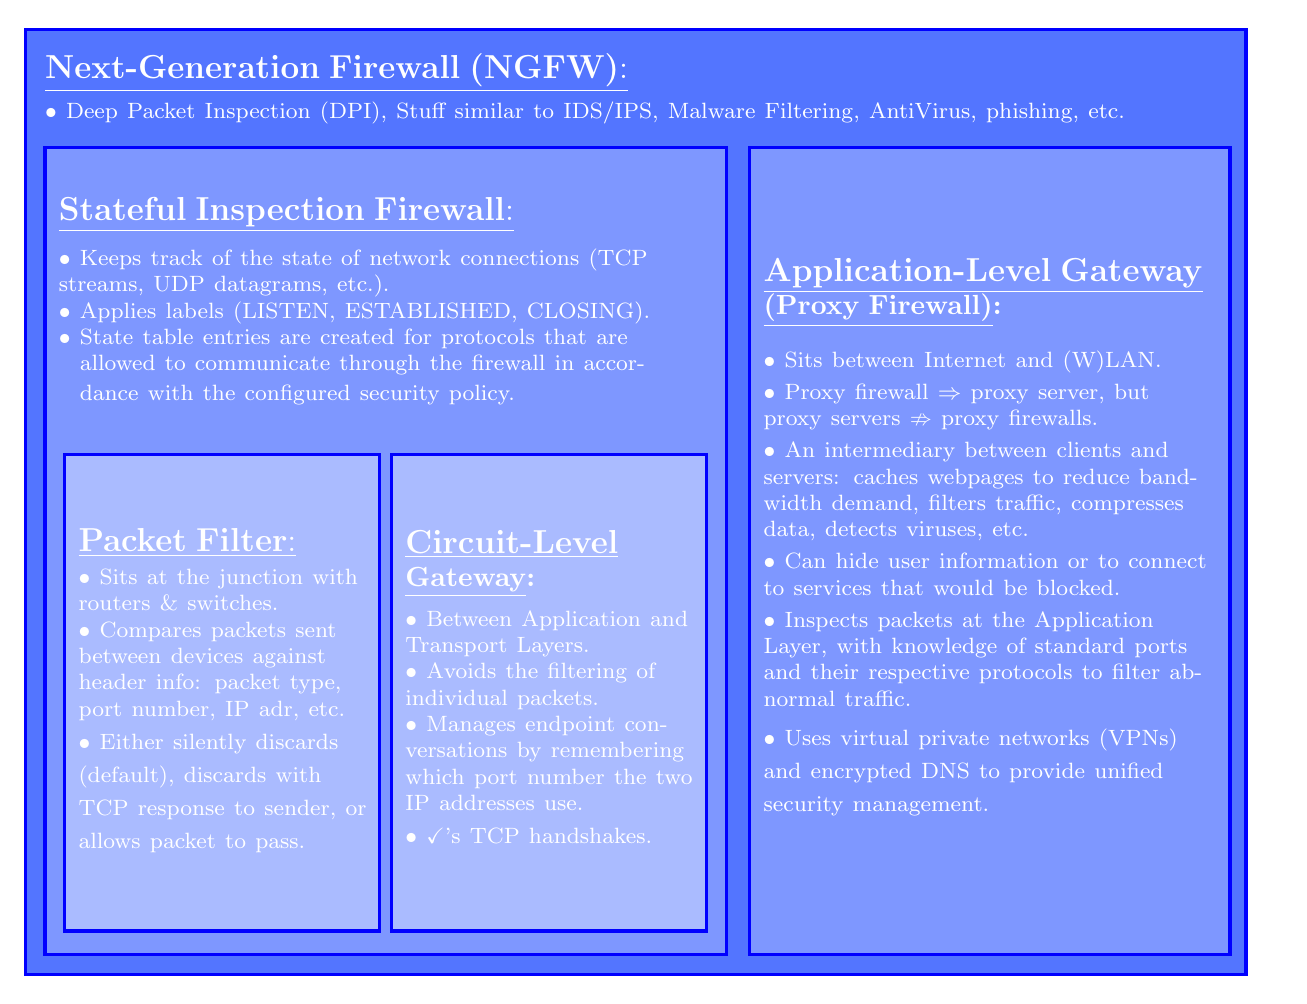
\begin{tikzpicture}
    \hspace{-0.05cm}\filldraw[color=blue, fill=blueone!90, very thick](0,0) rectangle (15.5,12);
    \node[text width=15.5cm] at (8, 11.25) {\textcolor{white}{\underline{\large\textbf{Next-Generation Firewall (NGFW)}:}\\
    \vspace{0.25em}
    \footnotesize $\bullet$ Deep Packet Inspection (DPI), Stuff similar to IDS/IPS, Malware Filtering, AntiVirus, phishing, etc.}};
        \begin{scope}[xshift = 0.25cm, yshift = 0.25cm]
            \filldraw[color=blue, fill=bluetwo!90, very thick](0,0) rectangle (8.65,10.25);
            \node[text width=8.25cm] at (4.3, 8.3) {\textcolor{white}{\underline{\large\textbf{Stateful Inspection Firewall}:}\\
            \vspace{0.5em}
            \footnotesize $\bullet$ Keeps track of the state of network connections (TCP streams, UDP datagrams, etc.). \\
            $\bullet$ Applies labels (LISTEN, ESTABLISHED, CLOSING). \\
            $\bullet$ State table entries are created for protocols that are \\
            \phantom{$\bullet$} allowed to communicate through the firewall in accor-\\
            \vspace{-0.15em}
            \phantom{$\bullet$} dance with the configured security policy.}};
            \begin{scope}[xshift = 0.25cm, yshift = 0.3cm]
                \filldraw[color=blue, fill=bluethree!90, very thick](0,0) rectangle (4,6.05);
                \node[text width=3.75cm] at (2.05, 3.05) {\textcolor{white}{\underline{\large\textbf{Packet Filter}:}\\
                \vspace{0.25em}
                \footnotesize $\bullet$ Sits at the junction with routers \& switches. \\
                $\bullet$ Compares packets sent between devices against header info: packet type, port number, IP adr, etc. \\
                $\bullet$ Either silently discards (default), discards with TCP response to sender, or allows packet to pass.}};
            \end{scope}
            \begin{scope}[xshift = 4.4cm, yshift = 0.3cm]
                \filldraw[color=blue, fill=bluethree!90, very thick](0,0) rectangle (4,6.05);
                \node[text width=3.75cm] at (2.05, 3.1) {\textcolor{white}{\underline{\large\textbf{Circuit-Level}} \\
                \textbf{\underline{Gateway}:}\\
                \vspace{0.5em}
                \footnotesize $\bullet$ Between Application and Transport Layers. \\
                $\bullet$ Avoids the filtering of individual packets. \\
                $\bullet$ Manages endpoint conversations by remembering which port number the two IP addresses use. \\
                $\bullet$ $\checkmark$'s TCP handshakes.}};
            \end{scope}
        \end{scope}
        \begin{scope}[xshift = 9.2cm, yshift = 0.25cm]
            \filldraw[color=blue, fill=bluetwo!90, very thick](0,0) rectangle (6.1,10.25);
            \node[text width=5.75cm] at (3.05, 5.3) {\textcolor{white}{\underline{\large\textbf{Application-Level Gateway}} \\
            \textbf{\underline{(Proxy Firewall)}:}\\
            \vspace{0.75em}
            \footnotesize $\bullet$ Sits between Internet and (W)LAN. \\
            \vspace{0.25em}
            $\bullet$ Proxy firewall $\Rightarrow$ proxy server, but proxy servers $\nRightarrow$ proxy firewalls. \\
            \vspace{0.25em}
            $\bullet$ An intermediary between clients and servers: caches webpages to reduce bandwidth demand, filters traffic, compresses data, detects viruses, etc.\\
            \vspace{0.25em}
            $\bullet$ Can hide user information or to connect to services that would be blocked. \\
            \vspace{0.25em}
            $\bullet$ Inspects packets at the Application Layer, with knowledge of standard ports and their respective protocols to filter abnormal traffic. \\
            \vspace{0.25em}
            $\bullet$ Uses virtual private networks (VPNs) and encrypted DNS to provide unified security management.}};
        \end{scope}
\end{tikzpicture}
\vspace{-1.5em}
\hspace{-0.06cm}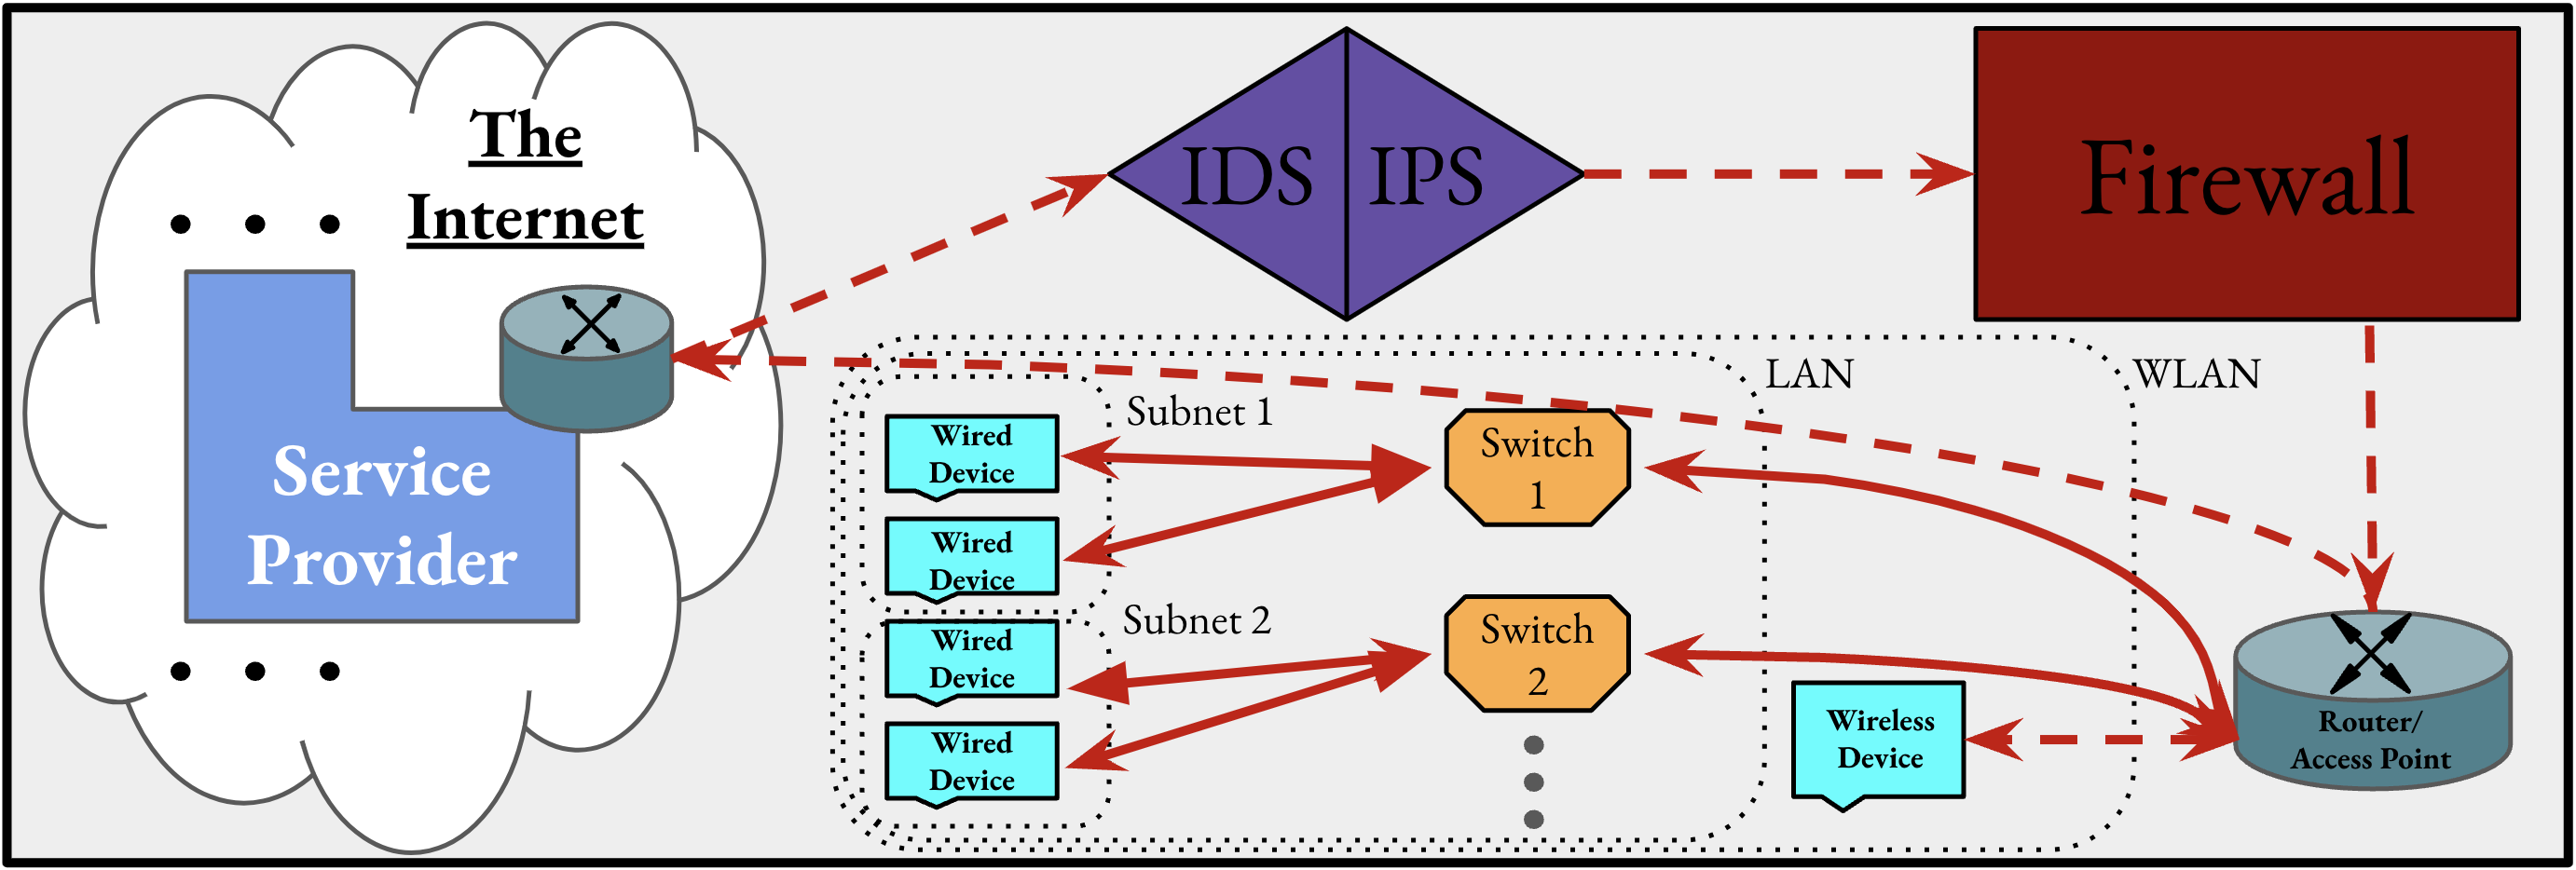
\includegraphics[width = 15.55cm, height = 6.05cm]{Network.png}
\end{center}
\vspace{0.5em}
\end{orangebox}

\begin{center}
\vspace{-0.25em}
\pgfornament[color=orange,width=1cm,ydelta=-10pt]{11}\pgfornament[color=orange,width=0.5cm,ydelta=-10pt]{6}\pgfornament[color=orange,width=1cm,ydelta=-10pt]{14}
\vspace{-0.4em}
\end{center}

\begin{orangebox}{Tuesday, June 6th}
This is my own box with a mandatory title.
\end{orangebox}

\begin{center}
\vspace{-0.25em}
\pgfornament[color=orange,width=1cm,ydelta=-10pt]{11}\pgfornament[color=orange,width=0.5cm,ydelta=-10pt]{6}\pgfornament[color=orange,width=1cm,ydelta=-10pt]{14}
\vspace{-0.4em}
\end{center}

\begin{orangebox}{Wednesday, June 7th}
This is my own box with a mandatory title.
\end{orangebox}

\begin{center}
\vspace{-0.25em}
\pgfornament[color=orange,width=1cm,ydelta=-10pt]{11}\pgfornament[color=orange,width=0.5cm,ydelta=-10pt]{6}\pgfornament[color=orange,width=1cm,ydelta=-10pt]{14}
\vspace{-0.4em}
\end{center}

\normalsize\begin{orangebox}{Thursday, June 8th}
This is my own box with a mandatory title.
\end{orangebox}

\begin{center}
\vspace{-0.25em}
\pgfornament[color=orange,width=1cm,ydelta=-10pt]{11}\pgfornament[color=orange,width=0.5cm,ydelta=-10pt]{6}\pgfornament[color=orange,width=1cm,ydelta=-10pt]{14}
\vspace{-0.4em}
\end{center}

\normalsize\begin{orangebox}{Friday, June 9th}
This is my own box with a mandatory title.
\end{orangebox}
\newpage

\noindent\begin{longfbox}[
rounded,
padding=4pt,
border-width=1.5pt,
border-top-left-radius=30pt,
border-left-width=8pt,
border-color=shininggold,
background-color=Lshininggold,
border-right-style=double,
]
\medskip
\phantom{~~}\Large\textbf{WEEK \barroman{IV}.} \large(06/12 - 06/16)\phantom{~~~~~~~~~~~~~~~~~~~~~~~~~~~~~~~~~~~~~~~~~~~~~~~~~~~~~~~~~~~~~~~~~~~~~~~~~~~~~~~~}
\end{longfbox}
\\

\begin{center}
\vspace{-1em}
\pgfornament[color=shininggold, width=6cm, ydelta=-10pt]{88}
\vspace{-0.5em}
\end{center}

\begin{shininggoldbox}{Monday, June 12th}
This is my own box with a mandatory title.
\end{shininggoldbox}

\begin{center}
\vspace{-0.25em}
\pgfornament[color=shininggold,width=1cm,ydelta=-10pt]{11}\pgfornament[color=shininggold,width=0.5cm,ydelta=-10pt]{6}\pgfornament[color=shininggold,width=1cm,ydelta=-10pt]{14}
\vspace{-0.4em}
\end{center}

\begin{shininggoldbox}{Tuesday, June 13th}
This is my own box with a mandatory title.
\end{shininggoldbox}

\begin{center}
\vspace{-0.25em}
\pgfornament[color=shininggold,width=1cm,ydelta=-10pt]{11}\pgfornament[color=shininggold,width=0.5cm,ydelta=-10pt]{6}\pgfornament[color=shininggold,width=1cm,ydelta=-10pt]{14}
\vspace{-0.4em}
\end{center}

\begin{shininggoldbox}{Wednesday, June 14th}
This is my own box with a mandatory title.
\end{shininggoldbox}

\begin{center}
\vspace{-0.25em}
\pgfornament[color=shininggold,width=1cm,ydelta=-10pt]{11}\pgfornament[color=shininggold,width=0.5cm,ydelta=-10pt]{6}\pgfornament[color=shininggold,width=1cm,ydelta=-10pt]{14}
\vspace{-0.4em}
\end{center}

\begin{shininggoldbox}{Thursday, June 15th}
This is my own box with a mandatory title.
\end{shininggoldbox}

\begin{center}
\vspace{-0.25em}
\pgfornament[color=shininggold,width=1cm,ydelta=-10pt]{11}\pgfornament[color=shininggold,width=0.5cm,ydelta=-10pt]{6}\pgfornament[color=shininggold,width=1cm,ydelta=-10pt]{14}
\vspace{-0.4em}
\end{center}

\begin{shininggoldbox}{Friday, June 16th}
This is my own box with a mandatory title.
\end{shininggoldbox}
\newpage

\noindent\begin{longfbox}[
rounded,
padding=4pt,
border-width=1.5pt,
border-top-left-radius=30pt,
border-left-width=8pt,
border-color=yellow,
background-color=Lyellow,
border-right-style=double,
]
\medskip
\phantom{~~}\Large\textbf{WEEK \barroman{V}.} \large(06/19 - 06/23)\phantom{~~~~~~~~~~~~~~~~~~~~~~~~~~~~~~~~~~~~~~~~~~~~~~~~~~~~~~~~~~~~~~~~~~~~~~~~~~~~~~~~}
\end{longfbox}
\\

\begin{center}
\vspace{-1em}
\pgfornament[color=yellow, width=6cm, ydelta=-10pt]{88}
\vspace{-0.5em}
\end{center}

\normalsize\begin{yellowbox}{Tuesday, June 20th}
This is my own box with a mandatory title.
\end{yellowbox}

\begin{center}
\vspace{-0.25em}
\pgfornament[color=yellow,width=1cm,ydelta=-10pt]{11}\pgfornament[color=yellow,width=0.5cm,ydelta=-10pt]{6}\pgfornament[color=yellow,width=1cm,ydelta=-10pt]{14}
\vspace{-0.4em}
\end{center}

\normalsize\begin{yellowbox}{Wednesday, June 21st}
This is my own box with a mandatory title.
\end{yellowbox}

\begin{center}
\vspace{-0.25em}
\pgfornament[color=yellow,width=1cm,ydelta=-10pt]{11}\pgfornament[color=yellow,width=0.5cm,ydelta=-10pt]{6}\pgfornament[color=yellow,width=1cm,ydelta=-10pt]{14}
\vspace{-0.4em}
\end{center}

\normalsize\begin{yellowbox}{Thursday, June 22nd}
This is my own box with a mandatory title.
\end{yellowbox}

\begin{center}
\vspace{-0.25em}
\pgfornament[color=yellow,width=1cm,ydelta=-10pt]{11}\pgfornament[color=yellow,width=0.5cm,ydelta=-10pt]{6}\pgfornament[color=yellow,width=1cm,ydelta=-10pt]{14}
\vspace{-0.4em}
\end{center}

\normalsize\begin{yellowbox}{Friday, June 23rd}
This is my own box with a mandatory title.
\end{yellowbox}
\newpage

\noindent\begin{longfbox}[
rounded,
padding=4pt,
border-width=1.5pt,
border-top-left-radius=30pt,
border-left-width=8pt,
border-color=leafgreen,
background-color=Lleafgreen,
border-right-style=double,
]
\medskip
\phantom{~~}\Large\textbf{WEEK \barroman{VI}.} \large(06/26 - 06/30)\phantom{~~~~~~~~~~~~~~~~~~~~~~~~~~~~~~~~~~~~~~~~~~~~~~~~~~~~~~~~~~~~~~~~~~~~~~~~~~~~~~~~}
\end{longfbox}
\\

\begin{center}
\vspace{-1em}
\pgfornament[color=leafgreen, width=6cm, ydelta=-10pt]{88}
\vspace{-0.5em}
\end{center}

\normalsize\begin{leafgreenbox}{Monday, June 26th}
This is my own box with a mandatory title.
\end{leafgreenbox}

\begin{center}
\vspace{-0.25em}
\pgfornament[color=leafgreen,width=1cm,ydelta=-10pt]{11}\pgfornament[color=leafgreen,width=0.5cm,ydelta=-10pt]{6}\pgfornament[color=leafgreen,width=1cm,ydelta=-10pt]{14}
\vspace{-0.4em}
\end{center}

\normalsize\begin{leafgreenbox}{Tuesday, June 27th}
This is my own box with a mandatory title.
\end{leafgreenbox}

\begin{center}
\vspace{-0.25em}
\pgfornament[color=leafgreen,width=1cm,ydelta=-10pt]{11}\pgfornament[color=leafgreen,width=0.5cm,ydelta=-10pt]{6}\pgfornament[color=leafgreen,width=1cm,ydelta=-10pt]{14}
\vspace{-0.4em}
\end{center}

\normalsize\begin{leafgreenbox}{Wednesday, June 28th}
This is my own box with a mandatory title.
\end{leafgreenbox}

\begin{center}
\vspace{-0.25em}
\pgfornament[color=leafgreen,width=1cm,ydelta=-10pt]{11}\pgfornament[color=leafgreen,width=0.5cm,ydelta=-10pt]{6}\pgfornament[color=leafgreen,width=1cm,ydelta=-10pt]{14}
\vspace{-0.4em}
\end{center}

\normalsize\begin{leafgreenbox}{Thursday, June 29th}
This is my own box with a mandatory title.
\end{leafgreenbox}

\begin{center}
\vspace{-0.25em}
\pgfornament[color=leafgreen,width=1cm,ydelta=-10pt]{11}\pgfornament[color=leafgreen,width=0.5cm,ydelta=-10pt]{6}\pgfornament[color=leafgreen,width=1cm,ydelta=-10pt]{14}
\vspace{-0.4em}
\end{center}

\normalsize\begin{leafgreenbox}{Friday, June 30th}
This is my own box with a mandatory title.
\end{leafgreenbox}
\newpage

\noindent\begin{longfbox}[
rounded,
padding=4pt,
border-width=1.5pt,
border-top-left-radius=30pt,
border-left-width=8pt,
border-color=hulkgreen,
background-color=Lhulkgreen,
border-right-style=double,
]
\medskip
\phantom{~~}\Large\textbf{WEEK \barroman{VII}.} \large(07/03 - 07/07)\phantom{~~~~~~~~~~~~~~~~~~~~~~~~~~~~~~~~~~~~~~~~~~~~~~~~~~~~~~~~~~~~~~~~~~~~~~~~~~~~~~~~}
\end{longfbox}
\\

\begin{center}
\vspace{-1em}
\pgfornament[color=hulkgreen, width=6cm, ydelta=-10pt]{88}
\vspace{-0.5em}
\end{center}

\normalsize\begin{hulkgreenbox}{Monday, July 3rd}
This is my own box with a mandatory title.
\end{hulkgreenbox}

\begin{center}
\vspace{-0.25em}
\pgfornament[color=hulkgreen,width=1cm,ydelta=-10pt]{11}\pgfornament[color=hulkgreen,width=0.5cm,ydelta=-10pt]{6}\pgfornament[color=hulkgreen,width=1cm,ydelta=-10pt]{14}
\vspace{-0.4em}
\end{center}

\begin{hulkgreenbox}{Wednesday, July 5th}
This is my own box with a mandatory title.
\end{hulkgreenbox}

\begin{center}
\vspace{-0.25em}
\pgfornament[color=hulkgreen,width=1cm,ydelta=-10pt]{11}\pgfornament[color=hulkgreen,width=0.5cm,ydelta=-10pt]{6}\pgfornament[color=hulkgreen,width=1cm,ydelta=-10pt]{14}
\vspace{-0.4em}
\end{center}

\begin{hulkgreenbox}{Thursday, July 6th}
This is my own box with a mandatory title.
\end{hulkgreenbox}

\begin{center}
\vspace{-0.25em}
\pgfornament[color=hulkgreen,width=1cm,ydelta=-10pt]{11}\pgfornament[color=hulkgreen,width=0.5cm,ydelta=-10pt]{6}\pgfornament[color=hulkgreen,width=1cm,ydelta=-10pt]{14}
\vspace{-0.4em}
\end{center}

\begin{hulkgreenbox}{Friday, July 7th}
This is my own box with a mandatory title.
\end{hulkgreenbox}
\newpage

\noindent\begin{longfbox}[
rounded,
padding=4pt,
border-width=1.5pt,
border-top-left-radius=30pt,
border-left-width=8pt,
border-color=oceanblue,
background-color=Loceanblue,
border-right-style=double,
]
\medskip
\phantom{~~}\Large\textbf{WEEK \barroman{VIII}.} \large(07/10 - 07/14)\phantom{~~~~~~~~~~~~~~~~~~~~~~~~~~~~~~~~~~~~~~~~~~~~~~~~~~~~~~~~~~~~~~~~~~~~~~~~~~~~~~~~}
\end{longfbox}
\\

\begin{center}
\vspace{-1em}
\pgfornament[color=oceanblue, width=6cm, ydelta=-10pt]{88}
\vspace{-0.5em}
\end{center}

\normalsize\begin{oceanbluebox}{Monday, July 10th}
This is my own box with a mandatory title.
\end{oceanbluebox}

\begin{center}
\vspace{-0.25em}
\pgfornament[color=oceanblue,width=1cm,ydelta=-10pt]{11}\pgfornament[color=oceanblue,width=0.5cm,ydelta=-10pt]{6}\pgfornament[color=oceanblue,width=1cm,ydelta=-10pt]{14}
\vspace{-0.4em}
\end{center}

\normalsize\begin{oceanbluebox}{Tuesday, July 11th}
This is my own box with a mandatory title.
\end{oceanbluebox}

\begin{center}
\vspace{-0.25em}
\pgfornament[color=oceanblue,width=1cm,ydelta=-10pt]{11}\pgfornament[color=oceanblue,width=0.5cm,ydelta=-10pt]{6}\pgfornament[color=oceanblue,width=1cm,ydelta=-10pt]{14}
\vspace{-0.4em}
\end{center}

\normalsize\begin{oceanbluebox}{Wednesday, July 12th}
This is my own box with a mandatory title.
\end{oceanbluebox}

\begin{center}
\vspace{-0.25em}
\pgfornament[color=oceanblue,width=1cm,ydelta=-10pt]{11}\pgfornament[color=oceanblue,width=0.5cm,ydelta=-10pt]{6}\pgfornament[color=oceanblue,width=1cm,ydelta=-10pt]{14}
\vspace{-0.4em}
\end{center}

\normalsize\begin{oceanbluebox}{Thursday, July 13th}
This is my own box with a mandatory title.
\end{oceanbluebox}

\begin{center}
\vspace{-0.25em}
\pgfornament[color=oceanblue,width=1cm,ydelta=-10pt]{11}\pgfornament[color=oceanblue,width=0.5cm,ydelta=-10pt]{6}\pgfornament[color=oceanblue,width=1cm,ydelta=-10pt]{14}
\vspace{-0.4em}
\end{center}

\normalsize\begin{oceanbluebox}{Friday, July 14th}
This is my own box with a mandatory title.
\end{oceanbluebox}
\newpage

\noindent\begin{longfbox}[
rounded,
padding=4pt,
border-width=1.5pt,
border-top-left-radius=30pt,
border-left-width=8pt,
border-color=blue,
background-color=Lblue,
border-right-style=double,
]
\medskip
\phantom{~~}\Large\textbf{WEEK \barroman{IX}.} \large(07/17 - 07/21)\phantom{~~~~~~~~~~~~~~~~~~~~~~~~~~~~~~~~~~~~~~~~~~~~~~~~~~~~~~~~~~~~~~~~~~~~~~~~~~~~~~~~}
\end{longfbox}
\\

\begin{center}
\vspace{-1em}
\pgfornament[color=blue, width=6cm, ydelta=-10pt]{88}
\vspace{-0.5em}
\end{center}

\normalsize\begin{bluebox}{Monday, July 17th}
This is my own box with a mandatory title.
\end{bluebox}

\begin{center}
\vspace{-0.25em}
\pgfornament[color=blue,width=1cm,ydelta=-10pt]{11}\pgfornament[color=blue,width=0.5cm,ydelta=-10pt]{6}\pgfornament[color=blue,width=1cm,ydelta=-10pt]{14}
\vspace{-0.4em}
\end{center}

\normalsize\begin{bluebox}{Tuesday, July 18th}
This is my own box with a mandatory title.
\end{bluebox}

\begin{center}
\vspace{-0.25em}
\pgfornament[color=blue,width=1cm,ydelta=-10pt]{11}\pgfornament[color=blue,width=0.5cm,ydelta=-10pt]{6}\pgfornament[color=blue,width=1cm,ydelta=-10pt]{14}
\vspace{-0.4em}
\end{center}

\normalsize\begin{bluebox}{Wednesday, July 19th}
This is my own box with a mandatory title.
\end{bluebox}

\begin{center}
\vspace{-0.25em}
\pgfornament[color=blue,width=1cm,ydelta=-10pt]{11}\pgfornament[color=blue,width=0.5cm,ydelta=-10pt]{6}\pgfornament[color=blue,width=1cm,ydelta=-10pt]{14}
\vspace{-0.4em}
\end{center}

\normalsize\begin{bluebox}{Thursday, July 20th}
This is my own box with a mandatory title.
\end{bluebox}

\begin{center}
\vspace{-0.25em}
\pgfornament[color=blue,width=1cm,ydelta=-10pt]{11}\pgfornament[color=blue,width=0.5cm,ydelta=-10pt]{6}\pgfornament[color=blue,width=1cm,ydelta=-10pt]{14}
\vspace{-0.4em}
\end{center}

\normalsize\begin{bluebox}{Friday, July 21st}
This is my own box with a mandatory title.
\end{bluebox}
\newpage

\noindent\begin{longfbox}[
rounded,
padding=4pt,
border-width=1.5pt,
border-top-left-radius=30pt,
border-left-width=8pt,
border-color=darkblue,
background-color=Ldarkblue,
border-right-style=double,
]
\medskip
\phantom{~~}\Large\textbf{WEEK \barroman{X}.} \large(07/24 - 07/28)\phantom{~~~~~~~~~~~~~~~~~~~~~~~~~~~~~~~~~~~~~~~~~~~~~~~~~~~~~~~~~~~~~~~~~~~~~~~~~~~~~~~~}
\end{longfbox}
\\

\begin{center}
\vspace{-1em}
\pgfornament[color=darkblue, width=6cm, ydelta=-10pt]{88}
\vspace{-0.5em}
\end{center}

\normalsize\begin{darkbluebox}{Monday, July 24th}
This is my own box with a mandatory title.
\end{darkbluebox}

\begin{center}
\vspace{-0.25em}
\pgfornament[color=darkblue,width=1cm,ydelta=-10pt]{11}\pgfornament[color=darkblue,width=0.5cm,ydelta=-10pt]{6}\pgfornament[color=darkblue,width=1cm,ydelta=-10pt]{14}
\vspace{-0.4em}
\end{center}

\normalsize\begin{darkbluebox}{Tuesday, July 25th}
This is my own box with a mandatory title.
\end{darkbluebox}

\begin{center}
\vspace{-0.25em}
\pgfornament[color=darkblue,width=1cm,ydelta=-10pt]{11}\pgfornament[color=darkblue,width=0.5cm,ydelta=-10pt]{6}\pgfornament[color=darkblue,width=1cm,ydelta=-10pt]{14}
\vspace{-0.4em}
\end{center}

\normalsize\begin{darkbluebox}{Wednesday, July 26th}
This is my own box with a mandatory title.
\end{darkbluebox}

\begin{center}
\vspace{-0.25em}
\pgfornament[color=darkblue,width=1cm,ydelta=-10pt]{11}\pgfornament[color=darkblue,width=0.5cm,ydelta=-10pt]{6}\pgfornament[color=darkblue,width=1cm,ydelta=-10pt]{14}
\vspace{-0.4em}
\end{center}

\normalsize\begin{darkbluebox}{Thursday, July 27th}
This is my own box with a mandatory title.
\end{darkbluebox}

\begin{center}
\vspace{-0.25em}
\pgfornament[color=darkblue,width=1cm,ydelta=-10pt]{11}\pgfornament[color=darkblue,width=0.5cm,ydelta=-10pt]{6}\pgfornament[color=darkblue,width=1cm,ydelta=-10pt]{14}
\vspace{-0.4em}
\end{center}

\normalsize\begin{darkbluebox}{Friday, July 28th}
This is my own box with a mandatory title.
\end{darkbluebox}
\newpage

\noindent\begin{longfbox}[
rounded,
padding=4pt,
border-width=1.5pt,
border-top-left-radius=30pt,
border-left-width=8pt,
border-color=indigo,
background-color=Lindigo,
border-right-style=double,
]
\medskip
\phantom{~~}\Large\textbf{WEEK \barroman{XI}.} \large(07/31 - 08/02)\phantom{~~~~~~~~~~~~~~~~~~~~~~~~~~~~~~~~~~~~~~~~~~~~~~~~~~~~~~~~~~~~~~~~~~~~~~~~~~~~~~~~}
\end{longfbox}
\\

\begin{center}
\vspace{-1em}
\pgfornament[color=indigo, width=6cm, ydelta=-10pt]{88}
\vspace{-0.5em}
\end{center}

\normalsize\begin{indigobox}{Monday, July 31st}
This is my own box with a mandatory title.
\end{indigobox}

\begin{center}
\vspace{-0.25em}
\pgfornament[color=indigo,width=1cm,ydelta=-10pt]{11}\pgfornament[color=indigo,width=0.5cm,ydelta=-10pt]{6}\pgfornament[color=indigo,width=1cm,ydelta=-10pt]{14}
\vspace{-0.4em}
\end{center}

\normalsize\begin{indigobox}{Tuesday, August 1st}
This is my own box with a mandatory title.
\end{indigobox}

\begin{center}
\vspace{-0.25em}
\pgfornament[color=indigo,width=1cm,ydelta=-10pt]{11}\pgfornament[color=indigo,width=0.5cm,ydelta=-10pt]{6}\pgfornament[color=indigo,width=1cm,ydelta=-10pt]{14}
\vspace{-0.4em}
\end{center}

\normalsize\begin{indigobox}{Wednesday, August 2nd}
This is my own box with a mandatory title.
\end{indigobox}





\end{document}
